
\documentclass[a4paper, oneside, 11pt]{report}
\usepackage{epsfig,pifont,float,multirow,amsmath,amssymb}
\newcommand{\mc}{\multicolumn{1}{c|}}
\newcommand{\mb}{\mathbf}
\newcommand{\mi}{\mathit}
\newcommand{\oa}{\overrightarrow}
\newcommand{\bs}{\boldsymbol}
\newcommand{\ra}{\rightarrow}
\newcommand{\la}{\leftarrow}
\usepackage{algorithm}
\usepackage{algorithmic}
\usepackage{hyperref}
\topmargin = 0pt
\voffset = -80pt
\oddsidemargin = 15pt
\textwidth = 425pt
\textheight = 750pt
\hypersetup{
    colorlinks=true,
    linkcolor=blue,
    filecolor=magenta,      
    urlcolor=cyan,
    pdftitle={Overleaf Example},
    pdfpagemode=FullScreen,
    }
\begin{document}

\begin{titlepage}
\begin{center}
\rule{12cm}{1mm} \\
\vspace{1cm}
{\large  CMP-6048A/7009A Advanced Programming} %Delete as appropriate
\vspace{7.5cm}
\\{\Large Project Report - 10 January 2024}
\vspace{1.5cm}
\\{\LARGE MATBAP: Maths Interpreter software} % You can add to this title of modify it if you wish
\vspace{1.0cm}
\\{\Large Group members: \\ Igor Stepanenko, Lyra, Liam Farese\ }
\vspace{10.0cm}
\\{\large School of Computing Sciences, University of East Anglia}
\\ \rule{12cm}{0.5mm}
\\ \hspace{8.5cm} {\large Version 2.0}
\end{center}
\end{titlepage}


\setcounter{page}{1}
%\pagenumbering{roman}
%\newpage


\begin{abstract}
Please replace this section with your own abstract. An abstract is a brief summary (maximum 250 words) of your entire project. It should cover your objectives, your methodologies used, a brief developmental history, your final results, in particular covering the optional tasks, and a discussion and conclusion. You do not cover the literature or background in an abstract nor should you use abbreviations or acronyms. The remainder of this report template has clear chapter titles and we suggest to stick to these although you can organise your material inside each chapter to your own preferences. A guideline in size is approximately 3,500 words (not including abstract, captions and references) but no real limit on figures, tables, diagrams, pseudo-code etc.
\end{abstract}

\chapter{Introduction}
\label{chap:intro}

The introduction should be brief and comprise the following:

\section{Project statement}
A (brief) statement including the nature of the project, i.e.\ what you will do, how you will accomplish it and what the final deliverable will be.

\section{Aims and objectives}

Clearly specify the main aim and objective(s) and subsequent tasks of your project. You can use a MoSCoW to further elaborate on each individual task. If you do so, use a table with three columns (e.g.\ Table \ref{Table1}), the first one having the four categories; the second column a brief description of the task and the third column further elaboration or comments on the task. Note that a MoSCoW is normally for functional requirements only. You should treat non-functional requirements in a separate MoSCoW.

\begin{table}[h]
\caption{MoSCoW}
\begin{center}
\begin{tabular}{|p{1in}|p{2in}|p{2.5in}|} \hline
Priority & Task & Comments \\ \hline \hline
\multirow{3}{1in}{Must}
& Task M1 & Comment M1 \\ \cline{2-3}
& Task M2 & Comment M2 \\ \cline{2-3}
& ... & ... \\ \hline \hline
\multirow{3}{1in}{Should}
& Task S1 & Comment S1 \\ \cline{2-3}
& Task S2 & Comment S2 \\ \cline{2-3}
& ... & ... \\ \hline \hline
\multirow{3}{1in}{Could}
& Task C1 & Comment C1 \\ \cline{2-3}
& Task C2 & Comment C2 \\ \cline{2-3}
& ... & ... \\ \hline \hline
\multirow{3}{1in}{Should not}
& Task SN1 & Comment SN1 \\ \cline{2-3}
& ... & ... \\ \hline
\end{tabular}
\label{Table1}
\end{center}
\end{table}


\chapter{Background}

Give a brief background on similar software, e.g.\ \cite{Desmos:2023}, \cite{Matlab:2023}, etc.
Also cite the books \cite{Nystrom:2021} or documentation \cite{WPF:2023} that you consulted.
You should add additional references to the corresponding bib file (References.bib) referred to in the bottom of this document.


\chapter{Development History}\label{Chap:DevHist}

linksDescribe the history of your development in terms of the iterations or sprints in your project (your Github repository or other version control should help you to retrospectively identify these). Use different sections for different sprints and subsections for specific details on the same sprint. Feel free to use subsubsections or paragraphs (which are not numbered) if needed. 

\% https://liamfarese.atlassian.net/browse/AP-8
\section{Sprint 1: Basic arithmetic calculations, Basic GUI.}
In our first sprint, we focused on building the foundation of our maths interpreter, like basic arithmetic calculations and basic GUI. Our objective was to develop a software that mathces the spec requirements and is a robust and scalable application, keeping in mind maintainability and testability.

\subsection{Lexer}
We developed a lexer that would tokenise expressions consisting of digits, binary operations, identifiers and functions like sin, cos and tan. One of the challenges we faced was unfamiliarity with F\# and functional programming, especially the recursive nature of this programming paradigm. 

\subsection{Parser}
We developed a parser that would parse and evaluate expressions that followed this basic grammar.
\begin{verbatim}
 <E>    ::= <T> <Eopt>
 <Eopt> ::= + <T> <Eopt> | - <T> <Eopt> | <empty>
 <T>    ::= <NR> <Topt>
 <Topt> ::= * <NR> <Topt> | / <NR> <Topt> | <empty>
 <NR>   ::= <int> | <float> | (E)
\end{verbatim}

\subsection{Basic GUI}
We used WPF\cite{WPF:2023} with C\# to develop a basic GUI, focusing on maintainability, testability, and scalability. App's architecture consists of several design patterns like Model-View-ViewModel\cite{MVVM:2022}, that improves GUI's responsiveness to user interactions and Dependency Injection\cite{DI:2023} for better modularity and easy maintenance. The GUI was a minimalistic interface allowing users to enter expressions and view the answers - see Figure \ref{basicgui}.

\subsection{Testing}
Thorough unit tests were written for both the C\# app and the F\# engine. Table \ref{sprint1-lexer-test} includes unit test for the Lexer. Table \ref{sprint1-parser-test} includes unit tests for the Parser. The table with GUI unit tests can be seen in \ref{sprint1-gui-test}. The use of the MVVM and Dependency Injection patterns allowed us to to use the Moq\cite{Moq} mocking library to mock Model behaviours in our ViewModel. This allowed us to test code in isolation without relying on behaviour of real dependencies and to have control over what is returned from the mocked methods. As a result our code coverage was above 80\%.

\subsection{Conclusion}
The first sprint laid a solid foundation for our maths interpreter. The lexer and parser were capable of evaluation basic arithmetic expressions and the GUI was providing simple interface for user interaction. Our testing strategy set a ensured that future features were build upon a reliable codebase. 

\section{Sprint 2: \href{https://liamfarese.atlassian.net/browse/AP-30}{As a user I want to have a basic GUI}}

\subsection{Updated GUI}

\subsection{Testing}

\section{Sprint 3: \href{https://liamfarese.atlassian.net/browse/AP-42}{As a user I want to be able to assign variables}}
\section{Sprint 4: \href{https://liamfarese.atlassian.net/browse/AP-50}{As a user I want to be able to plot lines and polynomials}}
\section{Sprint 5: As a developer I would like to have an AST Parser}
\section{Sprint 6: As a user I would like to run for-loops}
\section{Sprint 7: As a user I want to visualise an AST}
\section{Sprint n: And whatever we complete before we submit this}



\chapter{Final deliverable}\label{Impl}

In this chapter you cover the final or ``ultimate'' version of your project. It will show the final BNF, the final GUI, the architecture (which should be MVVM or MVC) that includes UML diagrams, additional algorithms if not already included in the previous sprint sections.

\section{Final BNF}

\section{Final GUI}

\section{Code architecture}

\section{Algorithms}

Algorithms can be described in this chapter if not already covered in previous sections. Pseudo-code is preferred over code snippets. If you use the latter then make sure it is well commented inside the code or via the figure caption. 

\begin{algorithm}[th]
\caption{ The Newton-Raphson method }
\begin{algorithmic}[1]
\STATE Initialise root based on estimate
\STATE Set stop criterion
\\ \texttt{const double error = 0.000001;}
\WHILE {stop criterion not met}
	\STATE Compute f(root)
	\STATE Compute f'(root)
	\STATE root := root - f(root)/f'(root)
\ENDWHILE
\end{algorithmic}
\end{algorithm}


Note that code snippets or lists of crucial programming code or large UML diagrams should go in Appendix \ref{app:other} (or further appendices).

\subsection{Testing}

Describe what testing you have done on the interpreter (lexer, parser and execution), GUI and GUI-Interpreter communication, plotting, etc. Table \ref{Table2} in Appendix \ref{app:test} should be completed to do basic arithmetic expression tests.


\chapter{Discussion, conclusion and future work}

Briefly discuss  your achievements and put them in perspective with the MoSCoW analysis you specified in Table \ref{Table1}. Also discuss future developments and how you see the deliverable improving if more time could be spent. Note that this section should not be used as a medium to vent frustrations on whatever did not work out (group issues, not enough time, illness, etc.) as this should be dealt with separately - keep it professional!


\bibliographystyle{apalike}
\raggedright
\bibliography{References}


\appendix
\chapter{Contributions}

State here the \% contribution to the project of each individual member of the group and describe in brief what each member has done (if this corresponds to particular sections in the report then please specify these).

\chapter{Testing}
\label{app:test}
\section{F\# engine unit testing}
\begin{table}[h]
\caption{Sprint 1, Lexer unit tests}
\label{sprint1-lexer-test}
\begin{tabular}{|l|l|l|}
\hline
\textbf{Expression}        & \textbf{Pass/Fail} & \textbf{Comment}                      \\ \hline
1a+12                      & Pass               & Tokenises variable, int and operation \\ \hline
33.3/(12 + 3.5a)           & Pass               & Float/Int distinct tokenisation       \\ \hline
sin(43)/cos(1.5) * tan(34) & Pass               & Function tokenisation                 \\ \hline
4 \% 2                     & Pass               & Modulus tokenisation                  \\ \hline
4\textasciicircum{}3       & Pass               & Power tokenisation                    \\ \hline
1. + 43                    & Pass               & Lexer error                           \\ \hline
1.4.2                      & Pass               & Lexer error                           \\ \hline
1\&                        & Pass               & Lexer error                           \\ \hline
\end{tabular}
\end{table}

\begin{table}[h]
\caption{Sprint 1, Parser unit tests}
\label{sprint1-parser-test}
\begin{tabular}{|l|l|l|}
\hline
\textbf{Expression} & \textbf{Pass/Fail} & \textbf{Comment}                                                                     \\ \hline
2+10                & Pass               & Parses and evaluates basic addition                                                  \\ \hline
7-3                 & Pass               & Parses and evaluates basic subtraction                                               \\ \hline
5*7                 & Pass               & \begin{tabular}[c]{@{}l@{}}Parses and evaluates basic \\ multiplication\end{tabular} \\ \hline
12/8                & Pass               & \begin{tabular}[c]{@{}l@{}}Parses and evaluates basic \\ division\end{tabular}       \\ \hline
5*2.3               & Pass               & Parses and evaluates integers with floats                                            \\ \hline
13.56-6+14*20.1     & Pass               & Order of operations                                                                  \\ \hline
5-2.5/(6.0+6.5)+1   & Pass               & Order of operations using brackets                                                   \\ \hline
1\&                 & Pass               & Operators without an operand between                                                 \\ \hline
6+-2                & Pass               & Operators without an operand between                                                 \\ \hline
5/                  & Pass               & Operator without an operand following                                                \\ \hline
*                   & Pass               & Operator with no operands at all                                                     \\ \hline
(()                 & Pass               & Opening a bracket without closing it                                                 \\ \hline
())                 & Pass               & Closing a bracket without having opened a matching one                               \\ \hline
1/0                 & Pass               & Division by 0                                                                        \\ \hline
\end{tabular}
\end{table}

\newpage
\section{C\# GUI unit testing}

\begin{table}[h]
\caption{Sprint 1, GUI unit test}
\label{sprint1-gui-test}
\begin{tabular}{|l|l|l|}
\hline
\textbf{Input} & \textbf{Pass/Fail} & \textbf{Comment}                 \\ \hline
123            & Pass               & Updates the View with user input \\ \hline
\end{tabular}
\end{table}


\section{Plot testing}

\chapter{GUI}
\label{app:gui}
\section{Basic GUI}
\begin{figure}[H]
\begin{center}
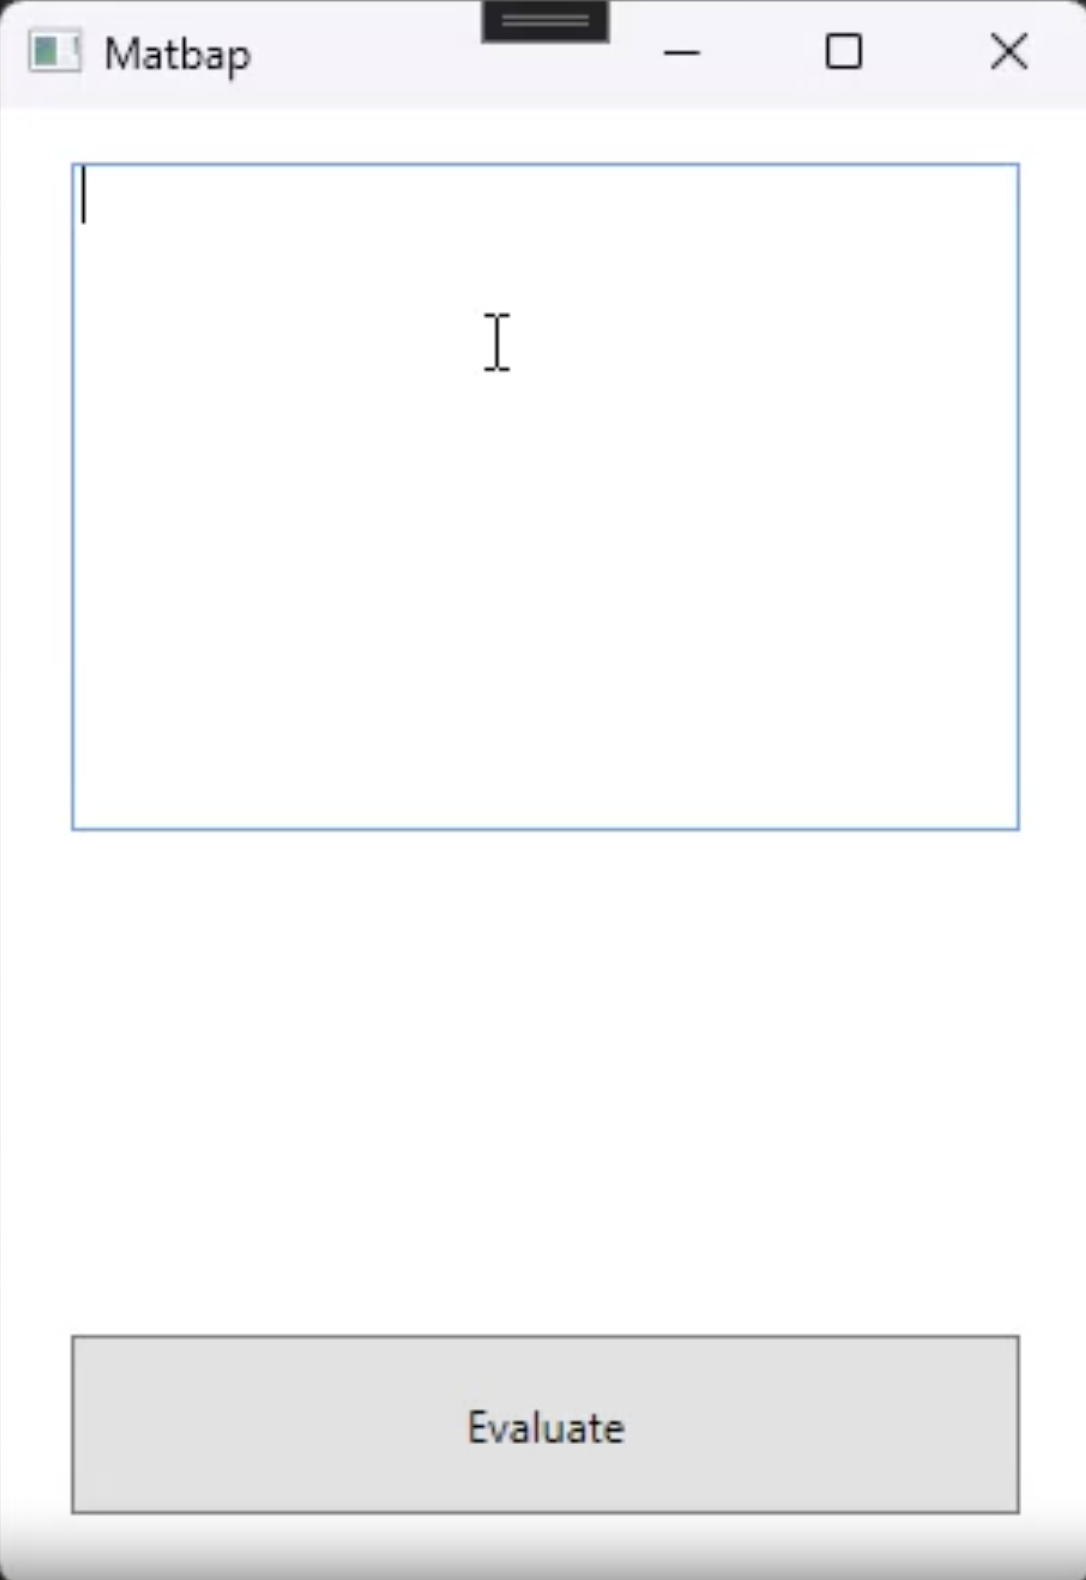
\includegraphics[scale=0.3 ]{Basic GUI.png}
\caption{Our first basic GUI}
\label{basicgui}
\end{center}
\end{figure}

\chapter{Other stuff}
\label{app:other}
\end{document}

